\documentclass[preprint,12pt]{elsarticle}

\usepackage{amsmath,amssymb}
\usepackage{graphicx}
\graphicspath{{../figures/}}
\usepackage{booktabs}
\usepackage[section]{placeins}
\renewcommand{\topfraction}{0.9}
\renewcommand{\bottomfraction}{0.8}
\renewcommand{\textfraction}{0.05}
\renewcommand{\floatpagefraction}{0.75}
\setcounter{topnumber}{3}
\setcounter{totalnumber}{5}
\usepackage{tikz}
\usetikzlibrary{positioning}
\usepackage[colorlinks=true,linkcolor=blue,citecolor=blue,urlcolor=blue]{hyperref}

\journal{Journal of Quantitative Spectroscopy and Radiative Transfer}

\begin{document}

\begin{frontmatter}

\title{Absolute sky radiance through deep twilight: a backward Monte
Carlo model with three-dimensional cloud transport, externally validated
to solar zenith angle 103 degrees}

\author[ku]{Mostafa Mahdi}
\affiliation[ku]{organization={University of Copenhagen},
            addressline={rhk510@alumni.ku.dk},
            city={Copenhagen},
            country={Denmark}}

\begin{abstract}
Deep twilight, solar zenith angles (SZA) between roughly $96^\circ$ and
$108^\circ$, is a difficult regime for radiative transfer: the line of
sight lies entirely inside the Earth's shadow, single scattering vanishes,
and the observable radiance is carried by multiply scattered light that has
crossed the terminator at high altitude. We present \textsf{twilight}, an
open-source backward Monte Carlo model that computes absolute spectral sky
radiance through this regime in a spherically stratified, refracting
atmosphere extending to 150~km, at 41 wavelengths with full Stokes
polarization, and with measured three-dimensional cloud fields traversed
voxel by voxel. Variance reduction combines forced collisions implemented
as truncated null-collision tracking against per-shell majorants,
collision-location importance sampling, directionally biased escape
sampling of the Dwivedi form, weight-window population control driven by a
deterministic solar-source importance map, hero-wavelength spectral
multiple importance sampling, and a bidirectional connection estimator
that couples every backward-chain collision to light subpaths traced from
the sunlit terminator, covering each scattering order beyond the second
from the sunlit side; each component is provably unbiased and the
implementation is held to that standard by analytic unit gates,
bit-identity harnesses, and statistical parity tests between four
independent implementations (scalar and polarized CPU chains, and Metal and
WGSL GPU kernels). Validation proceeds in three rings. Against reference
codes: absolute clear-sky radiance agrees with pseudospherical DISORT to
ratios of 0.975 to 0.993 at SZA $60^\circ$ to $85^\circ$;
144 of 144 cloud-slab comparison points agree with DISORT and MYSTIC within
3\% plus two standard errors; true-3D cloud cubes agree with SHDOM in 112
of 112 points; and cloud decks at twilight geometry are refereed against
MYSTIC runs of up to $10^9$ photons, to SZA $103^\circ$, with every cell
of the tier, one-dimensional and three-dimensional cloud paths alike,
statistically consistent with its reference (ratios 0.87 to 1.19).
Against measurements: the simulated zenith twilight decay reproduces
published sky-brightness data to 1.2 to 5.5\% per magnitude of decay.
Against human observation: a psychophysical detection layer, calibrated
once against a single regional campaign cluster, reproduces the dawn
detection times of sixteen published visual and instrumental campaigns
with a median absolute residual of $0.26^\circ$ of solar depression over
the fourteen scored rows, including an out-of-sample seasonal sweep at
$52^\circ$N. The
model, its validation caches, and every table in this paper are
reproducible from the public repository.
\end{abstract}

\begin{keyword}
radiative transfer \sep Monte Carlo \sep twilight \sep sky brightness \sep
polarization \sep three-dimensional clouds \sep visual detection
\end{keyword}

\end{frontmatter}

\section{Introduction}
\label{sec:intro}

The brightness of the twilight sky is one of the oldest quantitative
problems in atmospheric optics \citep{rozenberg1966}, and it remains one of
the least served by modern radiative transfer tools. The reason is
geometric. Once the Sun is more than about $6^\circ$ below the horizon, the
observer's entire line of sight lies inside the Earth's shadow; by
$12^\circ$ the shadow height above the observer exceeds the depth of the
dense atmosphere, and essentially no singly scattered photon can reach the
eye. What remains is light that was scattered at high altitude on the
sunlit side of the terminator, transported laterally over hundreds of
kilometers, and scattered again, possibly several times, into the line of
sight. Plane-parallel methods are structurally unable to represent this
transport; pseudospherical corrections extend them usefully to solar zenith
angles (SZA) near $90^\circ$ to $95^\circ$ but not beyond. Fully spherical
Monte Carlo codes such as MYSTIC \citep{mayer2009,emde2016} can in
principle go deeper, but published validation and practical convergence
reach SZA of roughly $100^\circ$; past that point the reference codes
themselves become the bottleneck.

Yet the deep-twilight regime is where several physically interesting and
socially important observables reside: the visual onset of dawn and the
disappearance of dusk colors (the basis of prayer timekeeping for roughly
two billion people), the visibility of the zodiacal light and its false
dawn, astronomical twilight for observatory scheduling, and the
photobiology of natural light exposure at high latitudes. All of these are
questions about absolute radiance in a regime where absolute radiance is
hard to compute and hard to validate.

This paper describes \textsf{twilight}, an open-source simulator built for
this regime, and the validation program that establishes what it can and
cannot currently claim. Three design decisions distinguish it from general-purpose
radiative transfer packages. First, the transport is backward
(adjoint) Monte Carlo from the observer, in a spherically stratified,
refracting atmosphere, with the entire sampling budget concentrated on the
multiply scattered field: the first scattering order is evaluated as an
exact deterministic integral, and the Monte Carlo estimator begins at order
two. Second, clouds are treated as measured three-dimensional fields, not
homogeneous layers: a georeferenced voxel volume, reconstructed from
geostationary satellite imagery by a neural network trained on spaceborne
cloud radar \citep{aybar2025}, is traversed exactly by the photon chains.
Third, the estimator stack was engineered specifically against the
heavy-tailed variance that dominates deep twilight, where the observable
mean is carried by rare chains that climb to the sunlit terminator; we
document both the machinery and its measured effect, including the
explicitly reported cases where affordable budgets remain statistically
weak.

A further methodological point deserves emphasis. Monte Carlo transport
codes fail most dangerously not by crashing but by converging confidently
to a biased answer; the literature of radiative transfer intercomparisons
is in large part a record of such discoveries. We therefore treat the
verification process itself as part of the model. Every estimator
component carries an analytic unit gate; every refactoring is pinned by
bit-identity harnesses over the unchanged surfaces; four independent
implementations (a scalar CPU chain, a polarized CPU chain, a Metal GPU
kernel, and a portable WGSL GPU kernel) are held in statistical parity
with pre-registered tolerance bands derived from measured seed variance;
and the code has twice been subjected to an adversarial review in which
independent re-derivations of the estimator mathematics hunted
specifically for compensating-error pairs. Findings from these reviews,
sixteen in the most recent round, all closed, are recorded in the
repository together with their fixes.

To state the contributions plainly: to our knowledge this work
provides (i) the deepest external radiative transfer comparison
attempted for cloud decks at twilight geometry (solar
zenith angle $103^{\circ}$ against $10^{9}$-photon MYSTIC references,
with every cell of the deep tier, one-dimensional and
three-dimensional field paths alike, gated and statistically
consistent;
published comparisons stop near $100^{\circ}$ under clear skies);
(ii) the only open transport code maintained as four parity-locked
implementations with pre-registered statistical acceptance bands;
(iii) the first twilight model validated simultaneously against
absolute pseudospherical reference codes, measured sky brightness, and a
century of human dawn observation; and (iv) a variance-reduction
stack whose measured effect in the heavy-tailed regime (a substantial
recovery of mean radiance in the deep broken-field cells, under a
verdict taxonomy that reports any non-constraining referee cell as
low-power rather than as agreement) is documented
alongside its mathematics.

Section~\ref{sec:model} describes the forward model: atmosphere,
scattering physics, background light sources, and the transport estimator.
Section~\ref{sec:variance} describes the variance-reduction stack and its
measured effect. Section~\ref{sec:gpu} describes the GPU implementations
and the cross-implementation parity methodology.
Section~\ref{sec:validation} presents the three-ring validation program:
reference codes, measured skies, and human observation campaigns.
Section~\ref{sec:uncertainty} describes the propagation of input
uncertainties to the output times. Section~\ref{sec:limits} states the
current limitations plainly, and Section~\ref{sec:conclusion} concludes.

\section{The forward model}
\label{sec:model}

\begin{figure}[t]
\centering
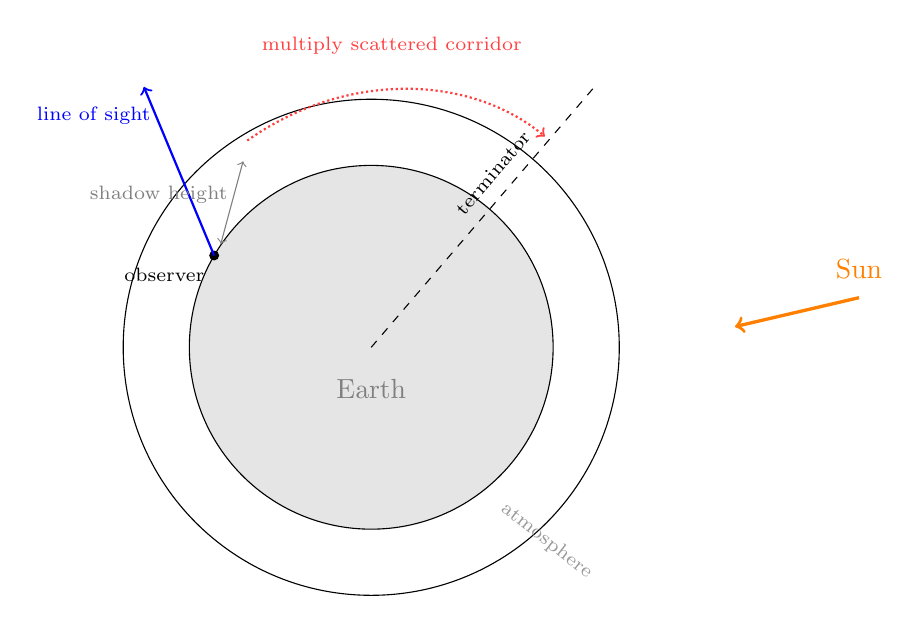
\begin{tikzpicture}[scale=1.05]
  % Earth and atmosphere
  \draw[fill=gray!20] (0,0) circle (2.2);
  \draw (0,0) circle (3.0);
  \node[gray] at (0,-0.5) {Earth};
  \node[gray!80, font=\scriptsize, rotate=-38] at (2.12,-2.34) {atmosphere};
  % Sun from the right
  \draw[->, very thick, orange] (5.9,0.6) -- (4.4,0.25);
  \node[orange] at (5.9,0.95) {Sun};
  % terminator
  \draw[dashed] (0,0) -- (2.7,3.15);
  \node[font=\scriptsize, rotate=49.4, above=1pt] at (1.62,1.95) {terminator};
  % observer on the night side (upper left)
  \filldraw (-1.9,1.11) circle (1.5pt);
  \node[font=\scriptsize, below left=0pt] at (-1.9,1.08) {observer};
  % line of sight
  \draw[->, thick, blue] (-1.9,1.11) -- (-2.75,3.15);
  \node[blue, font=\scriptsize, left] at (-2.55,2.8) {line of sight};
  % shadow height
  \draw[<->, gray] (-1.82,1.25) -- (-1.55,2.25);
  \node[gray, font=\scriptsize, left] at (-1.62,1.85) {shadow height};
  % corridor: climb, lateral at altitude, descend toward terminator
  \draw[->, red!75, thick, densely dotted]
    (-1.5,2.5) .. controls (-0.3,3.35) and (1.2,3.3) .. (2.1,2.55);
  \node[red!75, font=\scriptsize] at (0.25,3.65) {multiply scattered corridor};
\end{tikzpicture}
\caption{The deep-twilight geometry: beyond SZA ${\sim}96^{\circ}$ the
observer's entire line of sight lies inside the Earth's shadow; the
observable radiance is carried by photons scattered at high altitude
on the sunlit side of the terminator, transported laterally, and
scattered again into the line of sight (backward chains must discover
this corridor in reverse). Every variance-reduction component of
Section~\ref{sec:variance} exists to sample this corridor efficiently
without bias.}
\label{fig:geometry}
\end{figure}

\subsection{Atmosphere and optical properties}
\label{sec:atmosphere}

The atmosphere is represented by 56 concentric spherical shells extending
to 150~km, built on the US Standard Atmosphere 1976 with an extended
thermosphere. Shell boundaries are concentrated where the twilight
transport needs them: 1~km spacing in the troposphere and lower
stratosphere, coarsening upward. Molecular (Rayleigh) scattering follows
\citet{bodhaine1999}. Absorption includes five species: ozone
(Serdyuchenko cross sections, \citealp{serdyuchenko2014}), NO$_2$, the
O$_2$ bands, water vapor, and the O$_4$ collision-induced continuum, with
line data drawn from HITRAN \citep{gordon2022} and pre-integrated onto the
model's spectral grid. Aerosols follow the OPAC climatological types
\citep{hess1998}, scaled by a column optical depth that can be supplied
from measurement (Section~\ref{sec:uncertainty}). The spectral grid is 41
wavelengths from 380 to 780~nm, sufficient to resolve the Chappuis band of
ozone, whose absorption shapes twilight color.

Refraction is applied at every shell boundary by Snell's law on the local
radial gradient of refractive index; rays bend continuously in the
piecewise-constant-index limit, and total internal reflection (ducting) at
grazing incidence is handled explicitly. Refraction matters twice in this
regime: it lifts the apparent terminator, and it bends the long shadow-ray
paths that decide whether a scattering event is illuminated.

Clouds enter in two forms. A one-dimensional form treats a deck as a gray
extinction profile assigned to shells, with delta-Eddington scaling of the
optical depth and asymmetry parameter. The three-dimensional form is a
georeferenced voxel field of extinction and asymmetry (built from
the satellite reconstruction of \citealp{aybar2025}); chains
traverse it with an exact digital-differential-analyzer walk in the
style of \citet{amanatides1987} on the latitude, longitude, altitude grid, and
a two-level macrocell acceleration structure provides tile maxima for
majorant construction (Section~\ref{sec:forced}).

\subsection{Background light sources}
\label{sec:backgrounds}

At the depressions where dawn detection occurs, the twilight excess being
detected is comparable to, or below, the ambient night-sky radiance, so
the background must be modeled absolutely and per direction. The model
sums, for every simulated sky patch: zodiacal light from the measured
Leinert tables \citep{leinert1998} with the observer's heliocentric
geometry; integrated starlight from the Pioneer~10/11 photometry
\citep{toller1981}; airglow driven by the measured F10.7 solar radio flux;
moonlight following \citet{krisciunas1991}, supplied with the true lunar state
(parallax, phase angle, distance) from the JPL DE440 ephemeris
\citep{park2021}; and artificial skyglow from the propagated world atlas
\citep{falchi2016}, in its 2024 update, cross-checked against Visible
Infrared Imaging Radiometer Suite (VIIRS) nighttime lights, propagated
to the viewing geometry with a Garstang-type
model \citep{garstang1989}. The artificial veil is applied in mesopic
photometry computed from the source spectrum (high-pressure sodium versus
LED mixtures), because a fixed photopic conversion over-weights
sodium-dominated cities by more than a factor of two at threshold
adaptation levels \citep{cie191}.

\subsection{Solar geometry}

Solar position uses the NREL solar position algorithm (SPA)
\citep{reda2004}; when the DE440
kernel is available the Sun and Moon states are taken from the ephemeris
directly. The pipeline scans SZA rather than clock time and
converts the detected crossings back to time through the local solar
motion, which decouples the transport cache from date and longitude.

\subsection{Transport: exact first order plus backward Monte Carlo}
\label{sec:transport}

Radiance along the line of sight is split as $L = L_1 + L_{2+}$. The
single-scattering term $L_1$ is computed as a deterministic integral along
the refracted line of sight: at each quadrature point the direct solar
transmission is evaluated by a refracted shadow ray through the shell
stack (with the cloud field, when present, attenuating by Beer-Lambert
extinction along the exact voxel path), and the local phase matrix maps
the solar beam into the view direction. This term is exact up to
quadrature and dominates civil twilight.

The multiply scattered term $L_{2+}$ is estimated by backward Monte Carlo.
The line of sight is discretized into steps; from each step, secondary
chains are seeded by a three-component directional mixture (phase-function
proposal toward the Sun, a zenith-biased power-cosine lobe, and a
terminator-oriented lobe), extended by a fourth lateral-escape lobe that
activates only for cloud-coupled seeds under broken fields in the deep
regime (Section~\ref{sec:limits}), combined with a one-sample multiple importance
sampling (MIS) weight in the balance heuristic \citep{veach1995}, so the seed
estimator is unbiased for any mixture. Chains then propagate by free-path
sampling through the shell stack, scattering off the local
Rayleigh-plus-Henyey-Greenstein mixture, with polarization tracked by
Stokes vectors and the scattering-plane rotations applied in a fused form
that avoids explicit Mueller matrix products. At every collision a
next-event estimation shadow ray connects the chain to the Sun through the
refracting shells and the cloud field. Ground interaction is Lambertian
with configurable albedo, and ground-bounce next-event estimation is
included.

Under a three-dimensional cloud field the chain's free path is sampled
against a combined gas-plus-cloud channel. Because the voxel extinction is
not constant within a shell, the inversion uses null-collision (Woodcock)
tracking \citep{galtier2013} against per-shell majorants: tile maxima from
the macrocell structure, joined with the background column and rounded
upward so that single-precision domination is guaranteed. Real collisions
are classified gas versus cloud by the local extinction ratio; cloud
vertices scatter from the local delta-scaled asymmetry as a depolarizing
Henyey-Greenstein event. An equivalence gate (Section~\ref{sec:ring1})
verifies that a uniform field reproduces the one-dimensional deck chains
exactly.

Figure~\ref{fig:dop} shows the polarization output directly: the
degree of polarization of the multiply scattered zenith radiance
across the visible grid, carrying the expected rise with wavelength
as the Rayleigh single-scattering character strengthens.

\begin{figure}[t]
\centering
\includegraphics[width=0.62\textwidth]{p1_dop}
\caption{The degree of polarization of the backward Monte Carlo
zenith radiance is shown across the spectral grid at three SZA values
(clear sky, 40\,000 chains per wavelength). Deeper twilight requires
substantially larger budgets for per-wavelength polarization
convergence and is omitted.}
\label{fig:dop}
\end{figure}

\section{Variance reduction for the deep-twilight tail}
\label{sec:variance}

\begin{figure}[t]
\centering
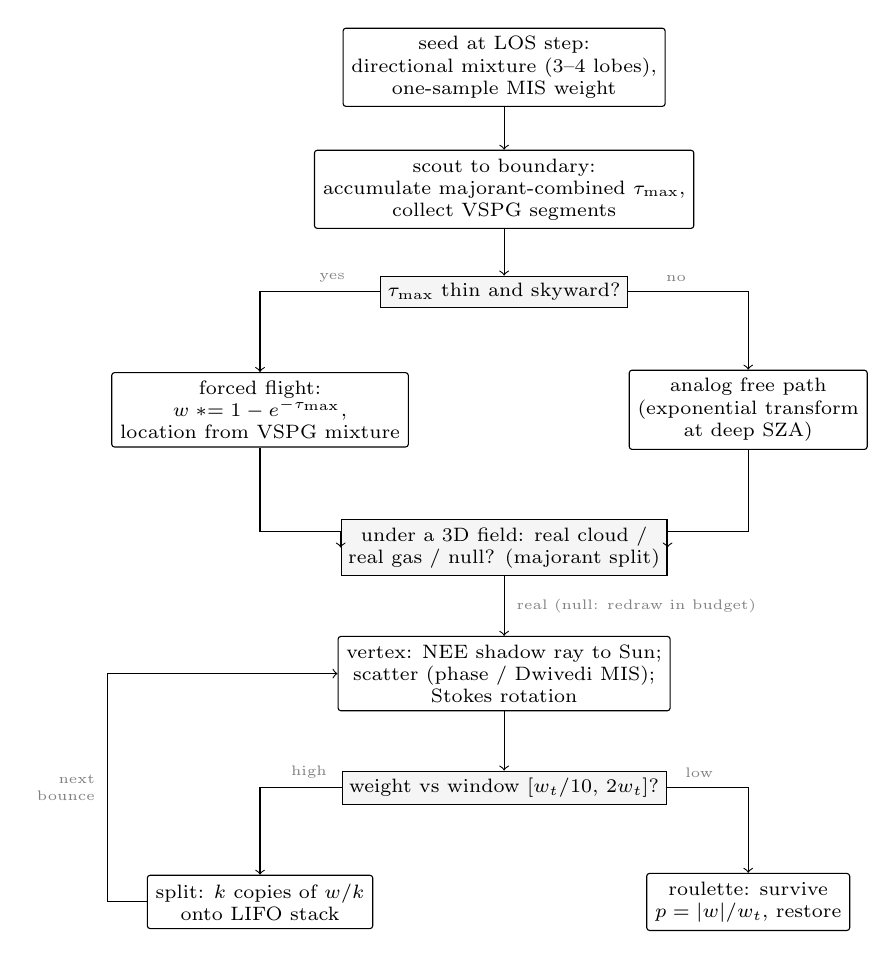
\begin{tikzpicture}[
  box/.style={draw, rounded corners=1pt, align=center,
              font=\scriptsize, inner sep=3pt},
  dec/.style={draw, align=center, font=\scriptsize, inner sep=2.5pt,
              fill=gray!8},
  lab/.style={font=\tiny, gray}]
  \node[box] (seed) at (0,0) {seed at LOS step:\\directional mixture (3--4 lobes),\\one-sample MIS weight};
  \node[box] (scout) at (0,-1.55) {scout to boundary:\\accumulate majorant-combined $\tau_{\max}$,\\collect VSPG segments};
  \node[dec] (forced) at (0,-2.85) {$\tau_{\max}$ thin and skyward?};
  \node[box] (ff) at (-3.1,-4.35) {forced flight:\\$w \mathrel{*}= 1-e^{-\tau_{\max}}$,\\location from VSPG mixture};
  \node[box] (analog) at (3.1,-4.35) {analog free path\\(exponential transform\\at deep SZA)};
  \node[dec] (null) at (0,-6.1) {under a 3D field: real cloud /\\real gas / null? (majorant split)};
  \node[box] (vertex) at (0,-7.7) {vertex: NEE shadow ray to Sun;\\scatter (phase / Dwivedi MIS);\\Stokes rotation};
  \node[dec] (ww) at (0,-9.15) {weight vs window $[w_t/10,\, 2w_t]$?};
  \node[box] (split) at (-3.1,-10.6) {split: $k$ copies of $w/k$\\onto LIFO stack};
  \node[box] (rr) at (3.1,-10.6) {roulette: survive\\$p = |w|/w_t$, restore};
  \draw[->] (seed) -- (scout);
  \draw[->] (scout) -- (forced);
  \draw[->] (forced.west) -| node[lab, above, pos=0.2]{yes} (ff.north);
  \draw[->] (forced.east) -| node[lab, above, pos=0.2]{no} (analog.north);
  \draw[->] (ff.south) |- ([yshift=2mm]null.west) -- (null.west);
  \draw[->] (analog.south) |- ([yshift=2mm]null.east) -- (null.east);
  \draw[->] (null) -- node[lab, right=1pt]{real (null: redraw in budget)} (vertex);
  \draw[->] (vertex) -- (ww);
  \draw[->] (ww.west) -| node[lab, above, pos=0.2]{high} (split.north);
  \draw[->] (ww.east) -| node[lab, above, pos=0.2]{low} (rr.north);
  \draw[->] (split.west) -- ++(-5mm,0) |- node[lab, left=1pt, pos=0.25, align=right]{next\\bounce} (vertex.west);
\end{tikzpicture}
\caption{The lifecycle of one secondary chain, showing where each
variance-reduction component of this section acts. Every branch is an
unbiased identity: forced flights and VSPG reweight the free-path
density, the null-collision loop telescopes to the analog
first-arrival law, the directional MIS uses the balance heuristic,
and splitting and roulette preserve expected weight.}
\label{fig:lifecycle}
\end{figure}

At SZA beyond about $100^\circ$ the estimator confronts a specific
pathology: almost all chains die in the dark, and the mean is carried by
rare chains that random-walk upward and sunward until they reach
illuminated altitudes. Left untreated, this produces heavy-tailed seed
distributions whose sample variance understates the true error, the most
dangerous failure mode a Monte Carlo code has, because it looks like
convergence. The stack described below was built against this failure
mode. Each component is
unbiased by construction; the telescoping identities are stated in the
code alongside the implementation and exercised by analytic unit gates.

\subsection{Forced collisions as truncated null-collision tracking}
\label{sec:forced}

Beyond SZA $96^\circ$ the free-path sampling is replaced, whenever the
path to the atmosphere boundary is optically thin, by a forced collision:
the chain weight is multiplied by $1 - e^{-\tau_{\max}}$ and the collision
optical depth is drawn from the truncated exponential on
$[0, \tau_{\max}]$. Under a cloud field, $\tau_{\max}$ is accumulated
against the majorant-combined channel, and the forced stage composes with
the null-collision classification: a drawn collision is real-cloud,
real-gas, or null in proportion to the local split
$\sigma_c(\mathbf{x}) : \sigma_g : (\bar\sigma - \sigma_c(\mathbf{x}))$,
and null events redraw within the remaining truncated budget. The product
of stage normalizers telescopes so that the sampled first-arrival law is
exactly the analog one; the identity is verified by a 400\,000-flight gate
against the analytic first-collision density on a checkerboard field,
under both tight and deliberately inflated ($\times 3$) majorants.

\subsection{Collision-location importance (VSPG)}

VSPG (volume scattering probability guiding) draws the collision
location of a forced flight from an importance mixture rather than
the bare truncated exponential.

Within a forced flight, the collision location is drawn not from the bare
truncated exponential but from a piecewise-exponential importance mixture
over the traversed shell segments, weighted by a calibrated function of
segment altitude and SZA that concentrates collisions where
the Sun still illuminates. The per-segment weights are collected during
the same shell walk that accumulates $\tau_{\max}$, at no additional traversal
cost. Buffer overflow on pathological multi-reflection paths extends the
final segment so the segment set always tiles $[0, \tau_{\max}]$,
preserving the exact normalization (an earlier silent truncation of this
buffer, which redistributed collision probability toward the path head, is
one of the compensating-error findings of the adversarial review).

\subsection{Directional biasing (Dwivedi) with balance-heuristic MIS}

Deep chains must travel laterally; an isotropizing phase function makes
lateral progress diffusive and slow. Following the deep-penetration
tradition of \citet{dwivedi1982}, a fraction of direction draws (ramped in
with SZA) samples a horizontally biased distribution in the local frame,
combined with the physical phase function through one-sample multiple
importance sampling so the estimator remains exactly unbiased. In the
polarized chain the balance-heuristic weight corrects the scalar
intensity; the Stokes rotation uses the actually sampled angle, so
polarization is transported without approximation.

\subsection{Weight windows, splitting, and a solar-source importance map}

Population control follows the weight-window formulation of the
deep-penetration literature \citep{wagner1998}: at each bounce the chain
weight is compared with a target derived from an importance function of
position; overweight chains split (each carrying weight $w/k$),
underweight chains face Russian roulette that restores survivors to the
target. Both operations are unbiased identities. The importance function
is supplied either by a calibrated altitude-plus-lateral heuristic or by a
deterministic solar-source map: in a spherically stratified atmosphere the
solar in-scatter density depends only on altitude and the cosine of the
position angle to the Sun, so a single $40 \times 64$ map, built per
radiance call from the local scattering coefficient times the
ground-shadow-aware solar transmittance and relaxed by a Bellman-Ford
transmittance recursion, serves every observer geometry. In measured
ledgers the map matches the tuned heuristic (evidence that the heuristic's
constants were near-optimal); it replaces hand tuning with physics and is
now the default. Figure~\ref{fig:imap} shows the map, and its near-uniformity is
itself a finding: above the boundary layer the atmosphere is
sufficiently transparent that nearly every cell in the domain can
reach sunlight at low optical cost, so the maximum-transmittance
importance saturates within roughly 30\% of unity everywhere except
the deepest low-altitude shadow. Population control keyed to any such
importance is therefore nearly inert in the deep regime, which is
precisely what the variance ledger measured (weight windows alone
left the deep-cell coefficient of variation unchanged); the binding
constraints are the collision-location and directional distributions,
not survival weighting.

\begin{figure}[t]
\centering
\includegraphics[width=0.72\textwidth]{p1_importance_map}
\caption{The deterministic solar-source importance map over altitude
and the cosine of the position angle to the Sun, on the production
clear-sky atmosphere at 450~nm (log scale, maximum normalized to
one; the dashed line marks the terminator). The map saturates near
unity through most of the domain because the upper atmosphere is
nearly transparent; the residual structure (about 30\%) sits in the
low-altitude deep shadow. This saturation explains the measured
result that weight windows alone do not reduce deep-twilight
variance: survival weighting has nothing to act on when almost every
position retains access to the sunlit source.}
\label{fig:imap}
\end{figure}

\subsection{Additional components}
\label{sec:components}

An exponential-transform path stretch biases free paths upward at deep
SZA with the standard weight correction. Spectrally, chains are traced at
a hero wavelength with adjoint-line-integration across the
41-wavelength grid: one geometric path is sampled using the hero
wavelength's optical properties, and its contribution is carried to
every other grid wavelength simultaneously by the ratio of
per-wavelength path transmittances to the hero's (exact, because the
path geometry is shared and only the extinction along it differs), so
a single walk services the full spectrum rather than 41 monochromatic
solves; the hero assignment rotates across chains and the estimates
combine by spectral multiple importance sampling in the style of
\citet{wilkie2014}; under
three-dimensional fields the per-wavelength chains run individually (the
per-wavelength null ratios under a shared majorant would otherwise be
heavy-tailed, a documented design deferral). A bidirectional subpath
reuse scheme contributes additional order-two connections on the main
chain. In the deep regime this generalizes to every higher order:
light subpaths traced from the sunlit top of the atmosphere maintain
a registry of 512 importance-weighted scatter vertices, and beyond
SZA $99^\circ$ every collision vertex of the backward chain
additionally makes a bidirectional connection to one registry vertex,
so that each scattering order of three and above receives a
contribution constructed from the sunlit side. At each order the
connection is combined with its next-event counterpart through a
per-path balance-heuristic multiple importance sampling weight; the
two weights are evaluated by one shared function and sum to unity, so
the combined estimator is unbiased by construction, and the
connection scores are normalized by the registry pass attempt count,
not by the count of successful connections. The scheme runs
identically on the scalar hero-wavelength chain and the polarized
Stokes chain, and a partition cross-check against the pre-connection
estimator agrees to 2.3\% at SZA $99.5^\circ$. Its effect is to
remove the dependence of the deep signal on rare long lateral random
walks; this is what resolves the one-dimensional SZA $103^\circ$
referee cells of Section~\ref{sec:cvresults}.

\subsection{Measured effect}
\label{sec:cvresults}

Table~\ref{tab:variance} reports the production estimator against the
MYSTIC references (standard errors 6 to 10\%) for the hardest
configuration we can referee externally: a uniform deck of
delta-scaled optical depth $\tau^{*} = 3$ under twilight geometry, at
1024 seeds of 16\,000 photons per wavelength (an eight-fold increase
over an earlier 128-seed pass). The regime is heavy-tailed. At this
budget the referee gates all six cells, and the
estimator is consistent with the reference in every one ($0.87$ to
$1.13\times$, bands $0.28$ to $0.40$); an apparent forty-percent-low
reading of the $550$~nm SZA $101^\circ$ cell at 128 seeds proved to be
seed undersampling of the heavy tail, not a bias, and resolved on
convergence. The three SZA $103^\circ$ cells, which under the purely
unidirectional estimator stayed heavy-tailed enough that the
confidence band remained above half the reference, gate once the
connection estimator of Section~\ref{sec:components} supplies each
scattering order of three and above from the sunlit side: across both
deck optical depths all six one-dimensional SZA $103^\circ$ cells
pass, with bands 0.31 to 0.40 of the reference and ratios 0.93 to
1.13. The two three-dimensional-field cells at SZA $103^\circ$, which
at their earlier 128-seed budget were reported low-power (consistent
but not constraining), close the same way the 128-seed deck cells
did, by seed statistics alone: at 1024 seeds ($\tau^{*}=1$) and 512
seeds ($\tau^{*}=3$) of 16\,000 photons the referee gates both, with
ratios 1.19 and 0.99 and bands 0.36 and 0.46 of the reference. The
connection estimator requires the one-dimensional combined channel
and deliberately leaves the field path untouched; the field cells
were closed with the field estimator unchanged, so the earlier
low-power verdicts were a statement about seed budget, not about the
estimator. The reference side was
itself replicated: eight fresh-seed $10^9$-photon MYSTIC replicas of
the four $\tau^{*}=3$ references reproduce the cached values within
their reported errors, except the 650~nm SZA $103^\circ$ case, whose
cached value sits 3.3 standard deviations below its two replicas (a
low draw); the model passes against both the cached and the
replica-pooled references. On a
synthetic broken-cloud field the same machinery drives a large recovery
of mean radiance relative to the analog estimator in the deep cells where
zenith starvation otherwise biases it low, with the seed coefficient of
variation reduced correspondingly; the per-configuration before-and-after
values are recorded in the archived field ledgers. On clear sky at
the dawn-detection
depressions the seed coefficient of variation improves by factors of two
to six.

\begin{table}[t]
\centering
\caption{Production estimator versus a $10^9$-photon MYSTIC referee.
Uniform cloud deck, delta-scaled optical depth $\tau^{*}=3$, zenith view,
1024 seeds of 16\,000 photons per wavelength. Ratios are model/referee;
uncertainties are seed standard errors. The referee gates a cell only
when the band $3\sqrt{\mathrm{se}^2+\mathrm{se}_{\mathrm{ref}}^2}+0.05\,r$
falls below half the reference $r$; cells above that are LOW-POWER
(consistent but not constraining) and reported as such rather than
counted as agreement. The analog-versus-stack variance recovery at
matched budget is Figure~\ref{fig:ledger}.}
\label{tab:variance}
\begin{tabular}{lccc}
\toprule
Cell (SZA / nm) & Estimator/referee & Band/referee & Verdict \\
\midrule
$101^\circ$ / 450 & $1.06\pm0.04\times$ & $0.28$ & consistent \\
$101^\circ$ / 550 & $0.87\pm0.05\times$ & $0.29$ & consistent \\
$101^\circ$ / 650 & $0.92\pm0.05\times$ & $0.30$ & consistent \\
$103^\circ$ / 450 & $0.94\pm0.05\times$ & $0.33$ & consistent \\
$103^\circ$ / 550 & $1.13\pm0.05\times$ & $0.38$ & consistent \\
$103^\circ$ / 650 & $1.09\pm0.05\times$ & $0.40$ & consistent \\
\bottomrule
\end{tabular}
\end{table}

\begin{figure}[t]
\centering
\includegraphics[width=\textwidth]{p1_variance_ledger}
\caption{Measured effect of the guiding stack on the seed coefficient
of variation. The left panel shows clear sky at the dawn-detection
depressions (16 seeds of 2\,000 chains per wavelength; labels give
SZA/nm); the right panel shows the uniform $\tau^{*}=3$ cloud field
(12 seeds of 4\,000 chains per wavelength). Gray bars show the analog
polarized chain before this work; blue bars show the full stack
(forced null-collision flights, VSPG, Dwivedi MIS, and weight
windows).}
\label{fig:ledger}
\end{figure}

\begin{figure}[t]
\centering
\includegraphics[width=\textwidth]{p1_deep_referee}
\caption{Every cell of the deep-regime referee table, shown as the
model-to-MYSTIC ratio with seed standard errors; referee budgets are
$3\times10^{8}$ to $10^{9}$ photons. All sixteen cells, the
one-dimensional and the three-dimensional field paths alike, are
gated and statistically consistent (green; ratios 0.87 to 1.19). The
two field cells at SZA $103^\circ$ that were low-power at 128 seeds
close at 1024 and 512 seeds with the field estimator unchanged.}
\label{fig:deep}
\end{figure}

Figure~\ref{fig:ledger} shows the ledger cell by cell, and
Figure~\ref{fig:deep} places every referee cell with its error bar.
Figure~\ref{fig:conv} shows the estimator's convergence across
budgets: at moderate depression the relative standard error follows
the $N^{-1/2}$ law from small budgets, while the deep cells show the
heavy-tail regime as departures from the ideal slope.

\begin{figure}[t]
\centering
\includegraphics[width=\textwidth]{p1_convergence}
\caption{Convergence of the production polarized estimator with chain
budget (clear sky, zenith view, 550~nm, SZA $97^{\circ}$, $101^{\circ}$,
and $103^{\circ}$, 12 seeds per point). The left panel shows the running
mean normalized to the largest budget, with seed standard errors; the
right panel shows the relative standard error against the ideal
$N^{-1/2}$ slope (dashed).}
\label{fig:conv}
\end{figure}

Two observations from this campaign generalize beyond our code. First,
the analog estimator (the before bars of Figure~\ref{fig:ledger})
illustrates the false-precision
failure: it returned 5 to 26\% of the true radiance with
deceptively tight seed spread, because no seed contained the rare
compensating chains. Sample variance is not a sufficient convergence
diagnostic in this regime; an external referee, or at minimum a
cross-estimator gate, is required. Second, population control and
directional guiding are not substitutes: weight windows alone (measured in
an intermediate ledger) left the coefficient of variation unchanged,
because splitting cannot multiply paths that the direction sampler never
generates; the directional component alone leaves the weight spread
untreated. The measured collapse in the coefficient of variation
required both components.

\section{Independent implementations and parity methodology}
\label{sec:gpu}

The estimator is implemented four times: a scalar CPU chain, the
production polarized CPU chain, a Metal shading language kernel, and a
WGSL kernel that runs on any Vulkan, DirectX~12, or Metal adapter through
the wgpu abstraction (this is the deployment path for headless Linux
servers). The GPU kernels implement the full stack including weight-window
splitting (a capped thread-local stack; the measured deep-cell effect
is given in Section~\ref{sec:limits}); buffer
layouts are shared byte-for-byte between the two shader languages and
pinned to the host by parse tests that read the shader source and compare
every offset constant against the packing code.

Parity between implementations is enforced statistically. For each gate
configuration (clear sky, uniform decks, checkerboard fields, a measured
field) the CPU reference and the GPU kernel are run over $K$ independent
seeds; the acceptance band on the ratio of means is derived from the
measured seed coefficients of variation before the comparison is made, and
the derivation is quoted in the gate's documentation. Bands that cannot
fail are treated as defects: an adversarial audit of the gate suite found
two such vacuous bands (one absolute band wider than the measured means,
one two-sided band wide enough to pass a 20\% bias) and both were
rewritten as ratio gates with bands that constrain. On current hardware the
Metal and wgpu backends agree with the CPU to ratios of 0.94 to 1.04 on
cloud fields and 0.995 to 1.010 on clear sky, with the GPU deep-field seed
coefficient of variation now below the CPU's own (the GPU kernels carry the
weight-window splitting and guiding stack; the forward-informed importance
map remains CPU-only, so the CPU stays the formal variance reference).
The bidirectional connection estimator of
Section~\ref{sec:components} likewise runs in the two CPU chains only;
the GPU kernels retain the pre-connection estimator, whose expectation is
identical, so the cross-implementation comparisons at deep solar zenith
angles remain statistical same-mean parities rather than draw-for-draw
identities, and the CPU chains carry the deep referee tier.

The portable WGSL path, which is the deployment route for non-Apple
servers, has been exercised on discrete NVIDIA silicon through Vulkan
rather than inferred from the Metal backend alone. On an NVIDIA~A10G
(driver reported through the Vulkan adapter) the full kernel suite passes
(125 of 125 gates) and clear-sky parity holds to ratios of 0.9993,
0.9963, and 0.9957 at zenith angles of $95^\circ$, $97^\circ$, and
$100^\circ$, matching the Apple figures to within their seed error. The
adversarial fine-checkerboard field gate evaluates the CPU and GPU means
at full dispatch size and gives a ratio of 1.35 at SZA $97^\circ$; its
acceptance band is wide (both estimators carry seed coefficients of
variation near 0.26 in this deep broken-field regime), so the band is
weak by construction, but it is derived from the measured seed dispersion
rather than inflated to pass, and the ratio sits at the upper documented
divergence of the GPU
deep-field case, where the CPU-only importance map is what tightens the
CPU reference (Section~\ref{sec:limits}); the clear-sky and
realistic-field paths, which are what a computed prayer day actually
traverses, are the tight ones.

\subsection{Computational cost}
\label{sec:perf}

A full computed prayer day (the complete depression scan with the
seven-patch detection fan, adaptive crossing refinement, and K-seed
repeats) costs 237~s on an Apple M2~Pro GPU (Metal) and 1585~s on its
eight performance cores (polarized CPU chains), with a scalar fast mode at
243~s; the numbers were measured under concurrent validation load and
are upper bounds, and the wgpu backend runs the same WGSL on headless
Vulkan hardware where dispatch shapes are not watchdog-limited: the
full-size checkerboard field gate, which the display-driven Apple GPU can
only bound from above before its watchdog intervenes, runs to completion
in 544~s on the headless A10G. The
referee side is far more expensive: the $10^{9}$-photon MYSTIC cells
of Section~\ref{sec:ring2} cost hours each on the same machine, which
is the practical argument for the estimator work of
Section~\ref{sec:variance}.

Beyond statistical parity, refactorings are pinned by bit-identity
harnesses: a dump of radiance bit patterns across a matrix of
configurations (clear sky, decks, fields, both chain families, multiple
scattering modes, a range of SZA) is compared between trees, and every
surface not intentionally changed must reproduce bit-for-bit. The
harness has caught, among other things, a random-number-stream
perturbation hidden behind an apparently neutral refactor. In the most
recent campaign, 984 of 984 unchanged rows were bit-identical, while the
one intentionally changed surface moved in all 82 of its rows.

\section{Validation}
\label{sec:validation}

The validation program is organized in three rings, from internal
exactness through external reference codes to human ground truth. All
referee caches (reference-code outputs, campaign run logs) are committed
to the repository, so every number below can be re-derived without
rebuilding the reference codes.

\subsection{Ring 1: internal exactness}
\label{sec:ring1}

Analytic unit gates verify each estimator identity in isolation: the
forced-flight first-arrival law against its closed form (per-bin agreement
at five standard errors across a fine checkerboard, under tight and
inflated majorants); majorant invariance (the estimate may not depend on
the looseness of the bound); the exact equivalence of a uniform voxel
field and the one-dimensional deck chains (0.04\% at matched seeds, and
ratio 0.999 to 1.000 in the dedicated deep-regime gate at SZA $101^\circ$
and $103^\circ$); the telescoping normalization of the VSPG segment set
($p_{\mathrm{sum}} \equiv 1-e^{-\tau_{\max}}$ to $10^{-12}$ on
200-traversal ducting paths); and the population-control identities.
Physics-constraint gates check monotonicity (radiance decreasing along
SZA ladders; the non-trivial ordering of clear versus thin-deck versus
thick-deck red-channel zenith radiance, where thin decks brighten the red
twilight zenith, a referee-corroborated finding) and smoothness (a
$\chi^2$ test across the forced-mode activation seam, which yields 11.6
on six degrees of freedom in the final configuration).

\subsection{Ring 2: reference codes and measured skies}
\label{sec:ring2}

\begin{table}[t]
\centering
\caption{Transport validation against reference codes and measured skies.
SE denotes standard error. The deep-regime rows are refereed by dedicated
MYSTIC runs of $3\times10^8$ to $10^9$ photons with standard errors of 6
to 10\%; the verdict taxonomy of Section~\ref{sec:cvresults} reports any
non-constraining cell as LOW-POWER rather than as agreement, and no cell
of the final campaign carries that label.}
\label{tab:refs}
\begin{tabular}{p{4.4cm}p{3.7cm}p{4.5cm}}
\toprule
Reference & Regime & Agreement \\
\midrule
DISORT, pseudospherical, 16 streams \citep{stamnes1988} & clear sky, SZA $60$ to $90^\circ$ & 2.6 to 3.5\% median (spectral shape) \\
DISORT, absolute scale & clear sky, SZA $60$ to $85^\circ$ & ratio 0.975 to 0.993 \\
MYSTIC, backward spherical MC \citep{mayer2009,emde2016} & clear sky, SZA $95$ to $100^\circ$, $10^8$ photons & 1 to 14\% \\
DISORT + MYSTIC, cloud slab & $\tau^{*} \in \{1, 3, 10\}$, SZA $30$ to $60^\circ$ & 144/144 points within 3\% + 2\,SE, both estimators \\
SHDOM, true-3D cubes \citep{evans1998} & checkerboard and broken deck & 64/64 and 48/48 points in band \\
MYSTIC, ultra-deep decks & $\tau^{*}$ 1 and 3, SZA $101$ to $103^\circ$, up to $10^9$ photons & all 16 cells, 1d and 3D-field, gated and consistent (ratios 0.87 to 1.19); the field cells closed by seed statistics at 1024 and 512 seeds \\
Measured zenith twilight decay \citep{patat2006,koomen1952} & civil through astronomical twilight & 1.2 to 5.5\% per magnitude of decay \\
\bottomrule
\end{tabular}
\end{table}

\begin{figure}[t]
\centering
\includegraphics[width=0.62\textwidth]{p1_clearsky_ratio}
\caption{The clear-sky model-to-referee radiance ratio versus SZA at
three wavelengths: the median and the 10 to 90\% spread over all view
geometries of the comparison bank (14\,486 points) are shown. The
referee is DISORT (pseudospherical) through SZA $90^{\circ}$ and MYSTIC
beyond.}
\label{fig:clearsky}
\end{figure}

\begin{figure}[t]
\centering
\includegraphics[width=0.55\textwidth]{p1_slab_scatter}
\caption{The cloud-slab bank compares both of the code's independent
Monte Carlo estimators with DISORT on the identical delta-scaled
Henyey-Greenstein problem (144 points across $\tau^{*} \in \{1, 3,
10\}$ and SZA $30$ to $60^{\circ}$, spanning three decades of
radiance). Dashed lines mark $\pm 3\%$.}
\label{fig:slab}
\end{figure}

Table~\ref{tab:refs} summarizes the reference-code ring;
Figures~\ref{fig:clearsky} and \ref{fig:slab} show the clear-sky ratio
bank and the cloud-slab scatter point by point,
Figure~\ref{fig:shdom} the true-3D cube comparison against SHDOM, and
Figure~\ref{fig:patat} the absolute comparison against the measured
Paranal twilight decay in both photometric bands.

\begin{figure}[t]
\centering
\includegraphics[width=0.6\textwidth]{p1_shdom}
\caption{The true-3D cloud cube comparison against SHDOM is shown
(checkerboard and broken-deck fields, both Monte Carlo estimators).
The shaded band marks $\pm 3\%$.}
\label{fig:shdom}
\end{figure}

\begin{figure}[t]
\centering
\includegraphics[width=0.68\textwidth]{p1_patat}
\caption{The absolute zenith twilight decay is compared with the
measured Paranal data of \citet{patat2006}: the engine V band (with the
site's measured night-sky floor added) and the twilight-only B band, in
magnitudes per square arcsecond, against the published quadratic fits
evaluated at integer zenith distances. Over ten magnitudes of decay the
engine tracks the measurement to 0.1 to 0.4~mag.}
\label{fig:patat}
\end{figure}

Three points
deserve comment. First, the absolute-scale DISORT comparison (no
normalization of any kind) is the anchor of the radiometric chain: ratios
0.975 to 0.993 across SZA $60^\circ$ to $85^\circ$ bound any calibration
error of the solar irradiance, cross sections, and quadrature at the
percent level. Second, the cloud-slab bank (144 points across three
optical depths, both of the code's independent Monte Carlo estimators,
against both DISORT and MYSTIC on the identical delta-scaled
Henyey-Greenstein problem) validates the cloud channel where the
references are strong, so that the twilight extension rests only on
geometry already validated in clear sky. Third, the ultra-deep rows
extend external refereeing to SZA $103^\circ$, which to our knowledge is
deeper than any published cloud-deck comparison (the complete
cell-by-cell table is given in Appendix~\ref{app:deep}). The two
three-dimensional-field cells at SZA $103^\circ$ were for some time
the statistically weak rows of this tier; larger seed campaigns (1024
seeds at $\tau^{*}=1$, 512 at $\tau^{*}=3$, of 16\,000 photons each)
closed them with the field estimator unchanged, confirming that the
earlier low-power verdicts measured the seed budget rather than the
estimator.

A note on reading ratios in the heavy-tailed regime is required,
because the deep rows can mislead in both directions. When the seed
distribution is dominated by rare bright chains, the sample mean at
affordable budgets sits below the true mean with high probability
(the typical seed misses the tail), so a ratio of, say, 0.6 with a
seed coefficient of variation near 100\% is what an unbiased
estimator is expected to show; it is not evidence of bias. Conversely,
a tight seed spread proves nothing if no seed contains the
compensating chains, as the analog before bars of
Figure~\ref{fig:ledger} demonstrate. Our acceptance bands therefore combine the referee's
standard error with the model-side seed spread, and rows whose bands
cannot constrain a meaningful bias are labeled LOW-POWER rather than
counted as agreement; the verdict taxonomy is applied mechanically,
before the numbers are seen.

\subsection{Ring 3: human observation campaigns}
\label{sec:ring3}

The application layer (described fully in a companion paper) converts
simulated radiance into detection times through a psychophysical
criterion. In brief: for each scanned depression the model simulates
five band patches across the dawn arch and two dark reference
patches; patch $i$ is distinct when its growth above its own
deep-night baseline exceeds the threshold set by the adaptation
luminance,
\begin{equation}
L_i(\theta) - B_i \ge f\, C_{\mathrm{thr}}(L_{\mathrm{ref}})\, L_{\mathrm{ref}},
\end{equation}
with $C_{\mathrm{thr}}$ the laboratory threshold-versus-intensity
function and $f$ a single calibrated field factor; dawn is declared
when the test passes across the band's lateral extent. In detail: seven simulated sky patches (five across the dawn band, two
dark references), Weber contrast of each band patch's growth above its own
deep-night baseline against threshold-versus-intensity data
\citep{blackwell1946,crumey2014}, with a single calibrated field factor
bridging laboratory detection of sharp-edged stimuli to field detection of
the borderless dawn gradient. For the purposes of the present paper, the
campaigns function as an end-to-end validation of the radiance model: if
the simulated absolute radiance, its spectral shape, and its spatial
gradient across the dawn band were wrong, no single constant could
reproduce detection times across sites, seasons, and latitudes.

Calibrated on the desert campaigns that report a documented central-mean
dawn, the model
reproduces sixteen published visual and instrumental campaigns, from a
1909 photographic
campaign at Aswan \citep{miethe1909} through the modern KACST desert
program \citep{almostafa2005}, the Hail campaign \citep{khalifa2018}, and
a calibrated-camera study \citep{mawad2024}, with a median absolute
residual of $0.26^\circ$ of solar depression over the fourteen scored
rows. The decisive out-of-sample
test is the OpenFajr program in Birmingham, UK \citep{openfajr2016}: 42
dated all-sky-camera series judged by a 19-member observer panel across a
full year at $52.4^\circ$N. The model, with zero retuning, reproduces the
panel's summer plateau (about $12.6^\circ$, deepening to $11.9^\circ$ at
the solstice, against 12.3 to $12.7^\circ$
observed) and the double-peaked seasonal curve, including the summer
relaxation that UK observers apply as an empirical rule; in the model it
emerges from persistent-twilight geometry, some twenty degrees of
latitude from the desert calibration campaigns.

The calibrated constant is fixed, and stress-tested, by inversion. The
published campaigns do not report a uniform statistic: several headline
depressions are documented upper bounds (mean or median plus one to two
standard deviations, the observing groups' stated ``highest value of
confidence''), not central means \citep{hassan2014,hassan2016}.
Restricted to the campaigns that report a genuine central mean --
Riyadh ($14.58^\circ$), Aswan ($14.90^\circ$), and Kottamia
($14.665^\circ$) -- the implied factor is 53, 51, and 57 (agreeing to
within four units of $f$), an optimum of $f=53$ with a plateau to 60; the production
constant is set to 56, within that band. Hail's central mean
($14.01^\circ$) is a half-degree shallower and implies $f\approx81$; an
earlier three-site cluster gave that lone anomaly a third of its weight
and was pulled to $f=70$. The remaining campaigns' headline values are
upper bounds whose raw central means (Tubruq $13.14^\circ$, Assiut
$11.25^\circ$) are far shallower and reflect all-nights or light-polluted
averages the clear-sky model does not represent; that the model at
$f=56$ reproduces the upper bounds is expected, since a site's
mean\,$+$\,2SD dawn is its deepest, clear-sky detection. The inversion
is latitude-independent.

\section{Input uncertainty propagation}
\label{sec:uncertainty}

Because the intended output is a time, the model propagates its input
uncertainties to a per-event standard deviation, reported alongside every
computed time. Three background terms are propagated through the measured
sensitivity of the detection margin at the crossing: the skyglow atlas
calibration (0.30 in log radiance), the street-light duty cycle (a bimodal
veil where part-night switching dominates the reference sky), and the
aerosol input (either a climatological bracket or the per-value envelope
of a measured product; the model ingests the Copernicus Atmosphere
Monitoring Service (CAMS) aerosol optical depth as an excess over a
baseline measured at the calibration sites). The realized
sensitivities validate against dedicated bracket campaigns: 13 to 17
degrees of depression per unit excess aerosol optical depth in the linear
regime, with the measured saturation behavior where the crossing slope
steepens. Representative outputs: a desert site reports $\pm 3.0$~min; a
mid-latitude winter city under sodium lighting reports $\pm 7.2$~min,
dominated by the street-light duty-cycle term, which no public data feed
currently supplies. We consider the width of these intervals
informative rather than a defect: a deterministic minute would
misrepresent what the inputs can support.

\section{Accuracy boundaries and open extensions}
\label{sec:limits}

Every boundary below is quantified, externally refereed where a
referee exists, and maintained as a living section of the repository
documentation; none affects the validated operating envelope of the
preceding sections. (i) The three-dimensional field path retains the
analog polarized chain: the Sun-side bidirectional connection
estimator of Section~\ref{sec:components}, which removes the
dependence of the deep signal on rare long lateral random walks,
requires the one-dimensional combined channel and does not yet extend
to heterogeneous voxel fields. The consequence is a convergence cost,
not a bias. The history of the deep tier is instructive here: an
eight-fold seed increase (to 1024 seeds) resolved every
one-dimensional SZA $101^\circ$ cell to referee consistency,
including the $550$~nm cell that at 128 seeds had read about forty
percent low (undersampling of the heavy tail, not a bias); the
one-dimensional SZA $103^\circ$ cells were then closed by the
connection estimator; and the two broken-field cells at SZA
$103^\circ$ ($\tau^{*} = 1$ and $3$, 550~nm), reported low-power at
128 seeds, pass the $10^9$-photon referee at 1024 and 512 seeds
respectively with the field estimator unchanged. The field path
therefore converges at practical budgets only through large seed
campaigns; extending the registry connections to voxel fields, which
would restore the one-dimensional convergence rate, is the identified
future work. Full bidirectional estimation had earlier been deferred
because multiple importance sampling weights in a refracting
spherical atmosphere carry a subtle-bias risk in precisely the regime
hardest to referee; the per-path shared-weight construction, whose
two weights sum to unity by evaluation of a single function, is what
made the combination safe to deploy on the one-dimensional channel.
(ii) Zenith views over broken cloud decks previously starved the
importance sampler; a lateral-escape seed lobe (an azimuthally
isotropic Dwivedi component folded into the seed mixture's
balance-heuristic MIS weight, active only for cloud-coupled seeds
under heterogeneous fields in the deep regime) closes the residual:
a gate-measured +14\% mean recovery with the seed coefficient of
variation halved at
SZA $100^{\circ}$, the restored zenith gate row passing two-sided,
and bit-identity preserved on every other surface (these are internal
gate diagnostics, since the analog reference here is noise-limited). The analog
reference above SZA $100^{\circ}$ over broken decks remains
noise-limited at affordable budgets, so the configuration is refereed
by the gate row rather than by analog parity. (iii) GPU kernels now carry the complete estimator stack including
weight-window splitting (a four-slot thread-local stack with the
CPU's roulette and split identities; measured on the uniform deck
gate, the deep-cell GPU seed coefficient of variation falls from
0.175 to 0.136, below the CPU's 0.269, with a 10 to 13 percent
wall-clock improvement as roulette kills outweigh split divergence);
the forward-informed importance map and the deeper CPU stack remain
CPU-only, so the CPU path stays the formal variance reference. (iv) Sea-horizon sites carry a
documented open offset: a one-dimensional aerosol column cannot
represent the directional marine boundary layer along the dawn path.
The voxel framework already accepts three-dimensional aerosol through
its gray extinction channel (a coastline-masked marine
boundary-layer field built this way is under evaluation), and a
spectral secondary aerosol grid would extend the per-shell majorants
additively, leaving the null-collision classification unchanged. (v) The evening red-twilight
(shafaq) calibration rests on instrumental rather than panel data, as no
color-resolved modern campaign exists. (vi) The model's own
field-instrument calibration campaign (a sky-quality-meter protocol
included with the code) has not yet begun; all human-observation validation is
against published campaigns.

\section{Conclusions}
\label{sec:conclusion}

We have described and validated an open-source backward Monte Carlo model
of absolute spectral sky radiance through deep twilight, with spherical
refracting geometry, full polarization, measured three-dimensional cloud
fields, and a variance-reduction stack engineered against the
heavy-tailed regime beyond SZA $100^\circ$. External refereeing now
reaches SZA $103^\circ$ on cloud decks at $10^9$ reference photons,
with every cell of the deep tier, one-dimensional and
three-dimensional field paths alike, gated and consistent (ratios
0.87 to 1.19);
absolute clear-sky radiance is anchored to DISORT at the percent level;
and the end-to-end chain, radiance through psychophysics, reproduces
sixteen human dawn-observation campaigns with a median absolute residual
of $0.26^\circ$ of depression over the fourteen scored rows, including a
year-long out-of-sample panel
study some twenty degrees of latitude from the desert calibration
campaigns.

\begin{table}[t]
\centering
\caption{The sixteen findings of the most recent adversarial review
round, by class, all closed before release. The compensating-error
findings are the class that neither unit tests nor aggregate validation
reliably catch.}
\label{tab:review}
\small
\setlength{\tabcolsep}{4pt}
\begin{tabular}{p{4.2cm}cp{6.6cm}}
\toprule
Class & Count & Representative finding \\
\midrule
Estimator (compensating-error) & 3 & importance-buffer overflow redistributing collision probability \\
Estimator (geometry/state) & 3 & detection fan frozen at the evening solar azimuth under three-dimensional fields \\
Photometry and inputs & 5 & photopic atlas value applied as a mesopic veil \\
Vacuous or mislabeled gates & 3 & absolute band wider than the measured means \\
Infrastructure & 2 & GPU seed salt discarded, collapsing repeat independence \\
\bottomrule
\end{tabular}
\end{table}

Beyond the specific results, we advocate two methodological
practices in radiative transfer code development (the yield of the
most recent review round is summarized in Table~\ref{tab:review}). First, pre-registered
statistical acceptance bands, derived from measured variance before the
comparison and audited for vacuousness, in place of informal agreement
plots. Second, adversarial review of estimator mathematics as a routine
phase: the compensating-error pairs that such review has twice found in
this code (a sub-surface ground-bounce misclassification masked by
near-cancellation; a silent importance-buffer truncation preserving total
probability while redistributing it) are precisely the class of defect
that neither unit tests nor aggregate validation reliably catch.

The simulator, the application layer, the validation caches, and the
scripts that regenerate every table in this paper are available in the
public repository; a versioned release accompanies this paper.

\appendix

\section{The complete deep-regime referee table}
\label{app:deep}

Table~\ref{tab:deepfull} lists every cell of the ultra-deep referee
comparison of Section~\ref{sec:ring2} with its budgets and verdicts,
as archived with the code release.

\begin{table}[h]
\centering
\caption{The complete deep-regime referee table, generated from the
archived comparison data: the 1d rows and the $\tau^{*}=1$ field rows
at 1024 seeds of 16\,000 photons per wavelength, the $\tau^{*}=3$
field rows at 512 seeds. tw is the model mean, CV
its per-seed coefficient of variation, and seeds the seed count; the
MYSTIC column gives the referee estimate and its photon budget.
Verdicts follow the taxonomy of Section~\ref{sec:ring2}. Radiances are
in W\,m$^{-2}$\,sr$^{-1}$\,nm$^{-1}$.}
\label{tab:deepfull}
\scriptsize
\setlength{\tabcolsep}{2.5pt}
\begin{tabular}{ccclccccccl}
\toprule
$\tau^{*}$ & SZA & nm & path & tw & CV [\%] & seeds & MYSTIC & photons & ratio & verdict \\
\midrule
% BEGIN GENERATED deep_table_body (scripts/make_tables.py)
1 & 101 & 450 & 1d & $1.51\times10^{-7}$ & 104 & 1024 & $1.53\times10^{-7}$ & $3\times10^{8}$ & 0.98 & PASS \\
1 & 101 & 550 & 1d & $1.16\times10^{-7}$ & 82 & 1024 & $1.16\times10^{-7}$ & $3\times10^{8}$ & 0.99 & PASS \\
1 & 101 & 550 & field & $1.37\times10^{-7}$ & 114 & 1024 & $1.16\times10^{-7}$ & $3\times10^{8}$ & 1.18 & PASS \\
1 & 101 & 650 & 1d & $7.92\times10^{-8}$ & 86 & 1024 & $8.78\times10^{-8}$ & $3\times10^{8}$ & 0.90 & PASS \\
1 & 103 & 450 & 1d & $2.55\times10^{-8}$ & 137 & 1024 & $2.73\times10^{-8}$ & $10^{9}$ & 0.93 & PASS \\
1 & 103 & 550 & 1d & $1.93\times10^{-8}$ & 147 & 1024 & $1.96\times10^{-8}$ & $10^{9}$ & 0.99 & PASS \\
1 & 103 & 550 & field & $2.32\times10^{-8}$ & 156 & 1024 & $1.96\times10^{-8}$ & $10^{9}$ & 1.19 & PASS \\
1 & 103 & 650 & 1d & $1.26\times10^{-8}$ & 121 & 1024 & $1.30\times10^{-8}$ & $10^{9}$ & 0.97 & PASS \\
3 & 101 & 450 & 1d & $1.33\times10^{-7}$ & 125 & 1024 & $1.26\times10^{-7}$ & $3\times10^{8}$ & 1.06 & PASS \\
3 & 101 & 550 & 1d & $1.07\times10^{-7}$ & 185 & 1024 & $1.22\times10^{-7}$ & $3\times10^{8}$ & 0.87 & PASS \\
3 & 101 & 550 & field & $1.11\times10^{-7}$ & 133 & 512 & $1.22\times10^{-7}$ & $3\times10^{8}$ & 0.91 & PASS \\
3 & 101 & 650 & 1d & $7.17\times10^{-8}$ & 162 & 1024 & $7.79\times10^{-8}$ & $3\times10^{8}$ & 0.92 & PASS \\
3 & 103 & 450 & 1d & $2.25\times10^{-8}$ & 166 & 1024 & $2.40\times10^{-8}$ & $10^{9}$ & 0.94 & PASS \\
3 & 103 & 550 & 1d & $1.70\times10^{-8}$ & 140 & 1024 & $1.51\times10^{-8}$ & $10^{9}$ & 1.13 & PASS \\
3 & 103 & 550 & field & $1.50\times10^{-8}$ & 224 & 512 & $1.51\times10^{-8}$ & $10^{9}$ & 0.99 & PASS \\
3 & 103 & 650 & 1d & $1.09\times10^{-8}$ & 143 & 1024 & $1.00\times10^{-8}$ & $10^{9}$ & 1.09 & PASS \\
% END GENERATED deep_table_body
\bottomrule
\end{tabular}
\end{table}

This table was re-measured on the final estimator: all sixteen rows
pass the gate. The two SZA $103^{\circ}$ field rows, low-power at the
earlier 128-seed budget, pass at 1024 and 512 seeds with the field
estimator unchanged, and no row carries the false-precision
signature of the analog estimator
(the pre-stack field estimator at $\tau^{*}=3$, SZA $103^{\circ}$ sat
at $0.13\times$ with a deceptively tight spread; the guided stack
replaces it with an honest, wider band). The one-dimensional cells of
Table~\ref{tab:variance} remain the tightest power statements.

\section*{Code and data availability}

The source code is available at
\url{https://github.com/Muno459/twilight} (dual-licensed
MIT/Apache-2.0); release v1.0.0 corresponds to this paper. The release
includes a validation archive containing the referee outputs, campaign
run records, and the exact data behind every figure and table of this
paper, together with the scripts that regenerate them.
Reference-code comparisons used libRadtran~2.0.6 (DISORT, MYSTIC) and
SHDOM. The three-dimensional cloud reconstruction uses the public
cloud3d network \citep{aybar2025}.

\section*{Funding and competing interests}

This research received no external funding. The author declares no
competing interests.

\section*{Acknowledgements}

The author thanks the maintainers of libRadtran and SHDOM, whose codes
served as referees, and the observers of the campaigns cited in
Section~\ref{sec:ring3}, whose patient observation of the dawn sky over
more than a century made the validation of Ring~3 possible.

\bibliographystyle{elsarticle-harv}
\begin{thebibliography}{00}

\bibitem[Al-Mostafa et al.(2005)]{almostafa2005}
Al-Mostafa, Z.A., et al., 2005. Studying of Twilight Project, first
part. Technical report, Institute of Astronomical and Geophysical
Research, King Abdulaziz City for Science and Technology (KACST),
Riyadh. One-year naked-eye and CCD morning-twilight campaign, deep
desert site 170~km from Riyadh.

\bibitem[Amanatides and Woo(1987)]{amanatides1987}
Amanatides, J., Woo, A., 1987. A fast voxel traversal algorithm for ray
tracing. In: Proceedings of Eurographics '87, pp. 3--10.

\bibitem[Aybar et al.(2025)]{aybar2025}
Aybar, C., et al., 2025. Cloud3D: neural reconstruction of
three-dimensional cloud structure from geostationary imagery trained on
CloudSat radar. arXiv:2511.04773.

\bibitem[Blackwell(1946)]{blackwell1946}
Blackwell, H.R., 1946. Contrast thresholds of the human eye. Journal of
the Optical Society of America 36, 624--643.

\bibitem[Bodhaine et al.(1999)]{bodhaine1999}
Bodhaine, B.A., Wood, N.B., Dutton, E.G., Slusser, J.R., 1999. On
Rayleigh optical depth calculations. Journal of Atmospheric and Oceanic
Technology 16, 1854--1861.

\bibitem[CIE(2010)]{cie191}
CIE, 2010. Recommended system for mesopic photometry based on visual
performance. CIE 191:2010, Commission Internationale de l'Eclairage,
Vienna.

\bibitem[Crumey(2014)]{crumey2014}
Crumey, A., 2014. Human contrast threshold and astronomical visibility.
Monthly Notices of the Royal Astronomical Society 442, 2600--2619.

\bibitem[Dwivedi(1982)]{dwivedi1982}
Dwivedi, S.R., 1982. A new importance biasing scheme for deep-penetration
Monte Carlo. Annals of Nuclear Energy 9, 359--368.

\bibitem[Emde et al.(2016)]{emde2016}
Emde, C., Buras-Schnell, R., Kylling, A., Mayer, B., Gasteiger, J.,
Hamann, U., Kylling, J., Richter, B., Pause, C., Dowling, T.,
Bugliaro, L., 2016. The libRadtran software package for radiative
transfer calculations (version 2.0.1). Geoscientific Model Development 9,
1647--1672.

\bibitem[Evans(1998)]{evans1998}
Evans, K.F., 1998. The spherical harmonics discrete ordinate method for
three-dimensional atmospheric radiative transfer. Journal of the
Atmospheric Sciences 55, 429--446.

\bibitem[Falchi et al.(2016)]{falchi2016}
Falchi, F., Cinzano, P., Duriscoe, D., Kyba, C.C.M., Elvidge, C.D.,
Baugh, K., Portnov, B.A., Rybnikova, N.A., Furgoni, R., 2016. The new
world atlas of artificial night sky brightness. Science Advances 2,
e1600377.

\bibitem[Galtier et al.(2013)]{galtier2013}
Galtier, M., Blanco, S., Caliot, C., Coustet, C., Dauchet, J.,
El~Hafi, M., Eymet, V., Fournier, R., Gautrais, J., Khuong, A.,
Piaud, B., Terr\'ee, G., 2013. Integral formulation of null-collision
Monte Carlo algorithms. Journal of Quantitative Spectroscopy and
Radiative Transfer 125, 57--68.

\bibitem[Garstang(1989)]{garstang1989}
Garstang, R.H., 1989. Night-sky brightness at observatories and sites.
Publications of the Astronomical Society of the Pacific 101, 306--329.

\bibitem[Gordon et al.(2022)]{gordon2022}
Gordon, I.E., et al., 2022. The HITRAN2020 molecular spectroscopic
database. Journal of Quantitative Spectroscopy and Radiative Transfer
277, 107949.

\bibitem[Hassan et al.(2014)]{hassan2014}
Hassan, A.H., Abdel-Hadi, Y.A., Issa, I.A., Hassanin, N.Y., 2014.
Naked-eye observations for morning twilight at different sites in Egypt.
NRIAG Journal of Astronomy and Geophysics 3, 23--26.

\bibitem[Hassan et al.(2016)]{hassan2016}
Hassan, A.H., Issa, I.A., Mousa, A.M., Abdel-Hadi, Y.A., 2016. Naked-eye
determination of the dawn for Sinai and Assiut of Egypt. NRIAG Journal
of Astronomy and Geophysics 5, 9--15.

\bibitem[Hess et al.(1998)]{hess1998}
Hess, M., Koepke, P., Schult, I., 1998. Optical properties of aerosols
and clouds: the software package OPAC. Bulletin of the American
Meteorological Society 79, 831--844.

\bibitem[Khalifa et al.(2018)]{khalifa2018}
Khalifa, N.S., Hassan, I.A., Taha, M.R., 2018. Naked-eye determination of
the solar depression angle of true dawn at Hail, Saudi Arabia. NRIAG
Journal of Astronomy and Geophysics 7, 22--26.

\bibitem[Koomen et al.(1952)]{koomen1952}
Koomen, M.J., Lock, C., Packer, D.M., Scolnik, R., Tousey, R.,
Hulburt, E.O., 1952. Measurements of the brightness of the twilight sky.
Journal of the Optical Society of America 42, 353--356.

\bibitem[Krisciunas and Schaefer(1991)]{krisciunas1991}
Krisciunas, K., Schaefer, B.E., 1991. A model of the brightness of
moonlight. Publications of the Astronomical Society of the Pacific 103,
1033--1039.

\bibitem[Leinert et al.(1998)]{leinert1998}
Leinert, C., et al., 1998. The 1997 reference of diffuse night sky
brightness. Astronomy and Astrophysics Supplement Series 127, 1--99.

\bibitem[Mawad(2024)]{mawad2024}
Mawad, R., 2024. The height of the diurnal atmosphere: twilight
altitude. Advances in Space Research 74.

\bibitem[Mayer(2009)]{mayer2009}
Mayer, B., 2009. Radiative transfer in the cloudy atmosphere. EPJ Web of
Conferences 1, 75--99.

\bibitem[Miethe and Lehmann(1909)]{miethe1909}
Miethe, A., Lehmann, E., 1909. D\"ammerungsbeobachtungen in Assuan,
Winter 1908. Meteorologische Zeitschrift 26.

\bibitem[OpenFajr(2016)]{openfajr2016}
OpenFajr Research Project, 2016. Research paper: an observational
study of the time of fajr in Birmingham, United Kingdom (May 2016,
with addendum September 2016).
\url{https://www.openfajr.org/docs/research_paper.pdf} (accessed
2026-07-06). All-sky CCD, 300 mornings; 42 clear-view series judged
by a 19-member consensus panel.

\bibitem[Park et al.(2021)]{park2021}
Park, R.S., Folkner, W.M., Williams, J.G., Boggs, D.H., 2021. The JPL
planetary and lunar ephemerides DE440 and DE441. The Astronomical
Journal 161, 105.

\bibitem[Patat et al.(2006)]{patat2006}
Patat, F., Ugolnikov, O.S., Postylyakov, O.V., 2006. UBVRI twilight sky
brightness at ESO-Paranal. Astronomy and Astrophysics 455, 385--393.

\bibitem[Reda and Andreas(2004)]{reda2004}
Reda, I., Andreas, A., 2004. Solar position algorithm for solar
radiation applications. Solar Energy 76, 577--589.

\bibitem[Rozenberg(1966)]{rozenberg1966}
Rozenberg, G.V., 1966. Twilight: A Study in Atmospheric Optics. Plenum
Press, New York.

\bibitem[Serdyuchenko et al.(2014)]{serdyuchenko2014}
Serdyuchenko, A., Gorshelev, V., Weber, M., Chehade, W., Burrows, J.P.,
2014. High spectral resolution ozone absorption cross-sections. Part 2:
temperature dependence. Atmospheric Measurement Techniques 7, 625--636.

\bibitem[Stamnes et al.(1988)]{stamnes1988}
Stamnes, K., Tsay, S.-C., Wiscombe, W., Jayaweera, K., 1988. Numerically
stable algorithm for discrete-ordinate-method radiative transfer in
multiple scattering and emitting layered media. Applied Optics 27,
2502--2509.

\bibitem[Toller(1981)]{toller1981}
Toller, G.N., 1981. A study of galactic light, extragalactic light, and
galactic structure using Pioneer 10 observations of background starlight.
Ph.D. thesis, State University of New York at Stony Brook.

\bibitem[Veach and Guibas(1995)]{veach1995}
Veach, E., Guibas, L.J., 1995. Optimally combining sampling techniques
for Monte Carlo rendering. In: Proceedings of SIGGRAPH '95, pp. 419--428.

\bibitem[Wagner and Haghighat(1998)]{wagner1998}
Wagner, J.C., Haghighat, A., 1998. Automated variance reduction of Monte
Carlo shielding calculations using the discrete ordinates adjoint
function. Nuclear Science and Engineering 128, 186--208.

\bibitem[Wilkie et al.(2014)]{wilkie2014}
Wilkie, A., Nawaz, S., Droske, M., Weidlich, A., Hanika, J., 2014. Hero
wavelength spectral sampling. Computer Graphics Forum 33, 123--131.

\end{thebibliography}

\end{document}
